\documentclass[11pt]{charter}

\usepackage{graphicx}
\usepackage{calc}
\usepackage[T1]{fontenc}

% El títulos de la memoria, se usa en la carátula y se puede usar el cualquier lugar del documento con el comando \ttitle
\titulo{Realidad Aumentada para la optimización de procedimientos \textit{batch} en la industria} 
	
% Nombre del posgrado, se usa en la carátula y se puede usar el cualquier lugar del documento con el comando \degreename
\posgrado{Carrera de Especialización en Sistemas Embebidos} 
%\posgrado{Carrera de Especialización en Internet de las Cosas} 
%\posgrado{Carrera de Especialización en Intelegencia Artificial}
%\posgrado{Maestría en Sistemas Embebidos} 
%\posgrado{Maestría en Internet de las cosas}

% Tu nombre, se puede usar el cualquier lugar del documento con el comando \authorname
\autor{Iván Szkrabko} 

% El nombre del director y co-director, se puede usar el cualquier lugar del documento con el comando \supname y \cosupname y \pertesupname y \pertecosupname
\director{Leandro Lanzieri}
\pertenenciaDirector{UTN} 
% FIXME:NO IMPLEMENTADO EL CODIRECTOR ni su pertenencia
\codirector{} % si queda vacio no se deberíá incluir 
\pertenenciaCoDirector{}

% Nombre del cliente, quien va a aprobar los resultados del proyecto, se puede usar con el comando \clientename y \empclientename
\cliente{Alejandro Carrasco}
\empresaCliente{ABB}

% Nombre y pertenencia de los jurados, se pueden usar el cualquier lugar del documento con el comando \jurunoname, \jurdosname y \jurtresname y \perteunoname, \pertedosname y \pertetresname.
\juradoUno{Nombre y Apellido (1)}
\pertenenciaJurUno{pertenencia (1)} 
\juradoDos{Nombre y Apellido (2)}
\pertenenciaJurDos{pertenencia (2)}
\juradoTres{Nombre y Apellido (3)}
\pertenenciaJurTres{pertenencia (3)}
 
\fechaINICIO{27 de junio de 2020}		%Fecha de inicio de la cursada de GdP \fechaInicioName
\fechaFINALPlanificacion{22 de Agosto de 2020} 	%Fecha de final de cursada de GdP
\fechaFINALTrabajo{22 de diciembre de 2020}		%Fecha de defensa pública del trabajo final


\begin{document}

\maketitle
\thispagestyle{empty}
\pagebreak


\thispagestyle{empty}
{\setlength{\parskip}{0pt}
\tableofcontents{}
}
\pagebreak


\section{Registros de cambios}
\label{sec:registro}


\begin{table}[ht]
\label{tab:registro}
\centering

\begin{tabularx}{\linewidth}{@{}|c|X|c|@{}}
\hline
\rowcolor[HTML]{C0C0C0} 
Revisión & \multicolumn{1}{c|}{\cellcolor[HTML]{C0C0C0}Detalles de los cambios realizados} & Fecha      \\ \hline
1.0      & Creación del documento                                                          & 27/06/2020 \\ \hline
1.1      & Primera versión, completo hasta punto 6                                                                                																						   & 10/07/2020 \\ \hline
1.2      & Completo hasta punto 11 																						   & 30/07/2020 \\ \hline
%1.2      & Otro ejemplo \newline
%		   Con texto partido \newline
%		   En varias líneas \newline
%		   A propósito                                                                     & dd/mm/aaaa \\ \hline
\end{tabularx}
\end{table}

\pagebreak



\section{Acta de constitución del proyecto}
\label{sec:acta}

\begin{flushright}
Buenos Aires, \fechaInicioName
\end{flushright}

\vspace{2cm}

Por medio de la presente se acuerda con el Ing.\authorname\hspace{1px} que su Trabajo Final de la \degreename\hspace{1px} se titulará ``\ttitle'', consistirá esencialmente en el prototipo preliminar de una aplicación de software para la supervisión y control de procesos \textit{batch} en la industria, y tendrá un presupuesto preliminar estimado de 640 hs de trabajo y \$ 2500, con fecha de inicio \fechaInicioName\hspace{1px} y fecha de presentación pública \fechaFinalName.

Se adjunta a esta acta la planificación inicial.

\vfill

% Esta parte se construye sola con la información que hayan cargado en el preámbulo del documento y no debe modificarla
\begin{table}[ht]
\centering
\begin{tabular}{ccc}
\begin{tabular}[c]{@{}c@{}}Ariel Lutenberg \\ Director posgrado FIUBA\end{tabular} &  & \begin{tabular}[c]{@{}c@{}}\clientename \\ \empclientename \end{tabular} \vspace{2.5cm} \\ 
\multicolumn{3}{c}{\begin{tabular}[c]{@{}c@{}} \supname \\ Director del Trabajo Final\end{tabular}} \vspace{2.5cm} \\
\begin{tabular}[c]{@{}c@{}}\jurunoname \\ Jurado del Trabajo Final\end{tabular}     &  & \begin{tabular}[c]{@{}c@{}}\jurdosname\\ Jurado del Trabajo Final\end{tabular}  \vspace{2.5cm}  \\
\multicolumn{3}{c}{\begin{tabular}[c]{@{}c@{}} \jurtresname\\ Jurado del Trabajo Final\end{tabular}} \vspace{.5cm}                                                                     
\end{tabular}
\end{table}




\section{Descripción técnica-conceptual del proyecto a realizar}
\label{sec:descripcion}

\begin{consigna}{black}
El presente proyecto consiste en desarrollar una interfaz de realidad aumentada, para que los operadores de plantas industriales puedan interactuar con un sistema de control distribuido de una manera practica e innovadora. La solución hace foco en la capacitación de los operadores, mediante el uso de rutinas \textit{batch}. Con el fin de guiarlos a través de los distintos procedimientos industriales, como pueden ser, arranques o paradas de emergencia en equipos críticos como hornos, calderas y reactores. La solución se implementara sobre un equipo de realidad aumentada de ultima tecnología de Microsoft denominado HoloLens2. Su plataforma de desarrollo se divide en dos áreas. Por un lado tenemos las interfaces visuales, las cuales se diseñan en Unity3D, que es una conocida plataforma para el desarrollo de videojuegos. Por otro lado tenemos el backend, este se desarrollara en .NET utilizando CSharp como lenguaje de programación. La aplicación embebida se comunicara con un servidor local a través de una APIrest, y desde el mismo se enviaran los datos pertinentes al sistema de control distribuido de ABB, a través del \textit{standard} industrial OPC (\textit{Open Platform Communications}).  

En la Figura \ref{fig:esquema_inicial} se puede observar de izquierda a derecha el flujo de la información, que comienza con un \textit{input} en la interfaz visual por parte del operador y termina con una acción determinada en el sistema de control.

\vspace{25px}

\begin{figure}[htpb]
    \centering
    \def\svgwidth{\columnwidth}
    \fontsize{8}{5}\fontencoding{T1}\fontfamily{lmss}\fontseries{eb}\selectfont
%	\def\svgscale{1}
    \input{Esquema_inicial.pdf_tex}
	\caption{Diagrama en bloques simplificado}
	\label{fig:esquema_inicial}
\end{figure}

\vspace{25px}

\end{consigna}


\section{Identificación y análisis de los interesados}
\label{sec:interesados}

\begin{consigna}{black} 
\begin{table}[ht]
%\caption{Identificación de los interesados}
%\label{tab:interesados}
\begin{tabularx}{\linewidth}{@{}|l|X|X|l|@{}}
\hline
\rowcolor[HTML]{C0C0C0} 
Rol           & Nombre y Apellido & Organización 	& Puesto 					\\ \hline
Auspiciante   & Víctor Toledo     & ABB         	& Gerente de Operaciones	\\ \hline
Cliente       & \clientename      &\empclientename	& Gerente de Ingeniería     \\ \hline
Impulsor      & Guillermo Lamana  & ABB           	& Project Manager       	\\ \hline
Responsable   & \authorname       & FIUBA        	& Alumno 					\\ \hline
Orientador    & \supname	      & \pertesupname 	& Director Trabajo final    \\ \hline
\end{tabularx}
\end{table}
 
Análisis de los interesados:
\begin{itemize}
\item Auspiciante: es riguroso y exigente con la utilización de los recursos y el tiempo.
\item Cliente: es detallista y busca que el producto sea perfecto.
\item Impulsor: es una persona que tiene además un rol de facilitador.
\item Orientador: será una fuente valiosa de consulta.
\end{itemize}

\end{consigna}



\section{1. Propósito del proyecto}
\label{sec:proposito}

\begin{consigna}{black}
El propósito de este proyecto es innovar en la interacción entre los operadores y los sistema de control distribuidos, para impulsar nuevas soluciones en el área de la automatización industrial. Se busca explorar las oportunidades que ofrece la realidad aumentada para mejorar y optimizar las tareas de los operadores, además de agilizar el entrenamiento de nuevos operarios y mejorar la seguridad para procedimientos bajo situaciones de emergencia.
\end{consigna}

\section{2. Alcance del proyecto}
\label{sec:alcance}

\begin{consigna}{black}
\textbf{El alcance del proyecto contempla:}
\begin{itemize}
\item Desarrollar una interfaz visual para el HoloLens2 que permita realizar el seguimiento de procesos \textit{batch} y rutinas de emergencia.
\item Desarrollar una interfaz de comunicación entre el HoloLens2 y un servidor web a través de una APIrest.
\item Desarrollar una interfaz de comunicación OPC entre el servidor web y el sistema de control.
\item Implementar lecturas de códigos QR para lograr el reconocimiento de equipos en planta.
\item Implementar un modo de visualización donde los elementos físicos de planta se complementen con la información del sistema de control, para indicar al operador el estado de cada elemento y sus propiedades en el sistema.
\item Implementar visualización de despieces mecánicos para guiar a los operadores en las tareas de mantenimiento.
\end{itemize}

\textbf{El alcance del proyecto no incluye:}
\begin{itemize}
\item Aquellas funcionalidades que no se encuentren contempladas dentro del alcance definido.
\end{itemize}
\end{consigna}


\section{3. Supuestos del proyecto}
\label{sec:supuestos}

\begin{consigna}{black}
Para el desarrollo del presente proyecto se supone que:

\begin{itemize}
\item Se dispone de 48 hs semanales para dedicar al desarrollo de la solución
\item Se tiene acceso al HoloLens2 durante el desarrollo de la solución
\end{itemize}

\end{consigna}

\section{4. Requerimientos}
\label{sec:requerimientos}

\begin{consigna}{black}
A continuación se listan los requerimientos en base a las distintas etapas de la solución:

\begin{enumerate}
\item Requerimientos asociados al desarrollo de la interfaz visual:
	\begin{enumerate}
	\item La interfaz debe ser intuitiva y simple.
	\item El idioma definido es ingles.
	\end{enumerate}
\item Requerimientos asociados al desarrollo de lógica en .NET:
	\begin{enumerate}
	\item La aplicación debe ser fluida y responder sin demoras apreciables por el operador, estableciéndose así el limite máximo de espera en 2 segundos.
	\item La aplicación debe poder hacer operaciones GET y POST sobre un servidor web, ya sea local o en la nube.
	\end{enumerate}
\item Requerimientos asociados a la API rest:
	\begin{enumerate}
	\item La API no sera de acceso publico, solo podrá ser consultada por las aplicaciones que poseen un \textit{token} de seguridad.
	\end{enumerate}
\item Requerimientos asociados a la interfaz de comunicación con el sistema de control:	
	\begin{enumerate}	
	\item La solución debe poder consultar una serie de datos específicos a elección, de los elementos que pertenecen al sistema de control.
	\item La comunicación debe cumplir con el \textit{standard} OPC.
	\end{enumerate}
\end{enumerate}

\end{consigna}

\section{5. Entregables principales del proyecto}
\label{sec:entregables}

\begin{consigna}{black}
Se entregarán los siguientes elementos:
\begin{itemize}
\item Manual de uso
\item Diagrama esquemático
\item Informe final
\end{itemize}

\end{consigna}

\section{6. Desglose del trabajo en tareas}
\label{sec:wbs}

\begin{consigna}{black}
Se divide el trabajo del proyecto en tareas y subtareas. Para facilitar el seguimiento, ninguna subtarea
consumirá más de 40 horas:

\begin{enumerate}
\item Investigación (Total: 24 hs)
	\begin{enumerate}
	\item Búsqueda de referencias a proyectos similares. (8 hs)
	\item Búsqueda y análisis de \textit{frameworks} útiles para desarrollar las soluciones.  (8 hs)
	\item Investigación de los servicios de Azure, para integrar al desarrollo. (8 hs)
	\end{enumerate}
\item Desarrollo de la interfaz visual: (Total: 88 hs)
	\begin{enumerate}
	\item Diseño de interfaz para la lectura de códigos QR. (16 hs)
	\item Diseño de interfaz para visualización de la información de los elementos del sistema de control. (16 hs)
	\item Diseño de interfaz para guiar al operador a través de los distintos pasos del procedimiento \textit{batch}. (40 hs)
	\item Pruebas, correcciones y mejoras. (16 hs)
	\end{enumerate}
\item Desarrollo de la lógica para la interfaz visual: (Total: 136 hs)
	\begin{enumerate}
	\item Desarrollo de la lógica para realizar las lecturas de códigos QR. (40 hs)
	\item Desarrollo de la lógica para realizar la interacción del operador con los datos del sistema. (32 hs)
	\item Desarrollo de la lógica para guiar al operador a través de los distintos pasos del procedimiento \textit{batch}. (32 hs)
	\item Pruebas, correcciones y mejoras. (32 hs)
	\end{enumerate}
\item Desarrollo de la API Rest (Total: 152 hs)
	\begin{enumerate}
	\item Investigación de distintas tecnologías. (16 hs)
	\item Desarrollo de la solución:
		\begin{enumerate}
			\item Programación de \textit{endpoints}. (40 hs)
			\item Implementación de medidas de seguridad de la API. (40 hs)
			\item \textit{Hosting} de la API. (40 hs)
		\end{enumerate}
	\item Pruebas, correcciones y mejoras. (16 hs)
	\end{enumerate}
\item Desarrollo de la interfaz de comunicación OPC (Total: 160 hs)
	\begin{enumerate}
	\item Investigación de \textit{frameworks} y análisis del protocolo (40 hs)
	\item \textit{Deploy} del cliente OPC (40 hs)
	\item Desarrollo de la comunicación con el server OPC (40 hs)
	\item Pruebas, correcciones y mejoras. (40 hs)
	\end{enumerate}

\item Pruebas integrales (Total: 32 hs)

\item Documentación (Total: 32 hs)

\item Presentaciones al cliente (Total: 16 hs)
\end{enumerate}

Cantidad total de horas: (640 hs) 

\end{consigna}

\section{7. Diagrama de Activity On Node}
\label{sec:AoN}

\begin{consigna}{black}
Los tiempos de las tareas en la Figura \ref{fig:aon} se encuentran expresados en horas:

\begin{figure}[H]
    \centering
    \def\svgwidth{\columnwidth}  
    \fontsize{7}{5}\fontencoding{T1}\fontfamily{lmss}\fontseries{eb}\selectfont
%	\def\svgscale{1}
    \input{aon.pdf_tex}
	\caption{Diagrama Activity On Node}
	\label{fig:aon}
\end{figure}

En el AON se marco con color rojo el considerado camino critico del proyecto. Si bien hay un conjunto de tareas en paralelo a lo largo del camino critico, las tareas que atraviesa son las que se consideran de mayor riesgo y dificultad. 

\end{consigna}

\section{8. Diagrama de Gantt}
\label{sec:gantt}

\begin{consigna}{black}
Se elaboro el siguiente diagrama considerando una cantidad de 15 horas semanales efectivas de trabajo:

\begin{figure}[H]
 \centering
 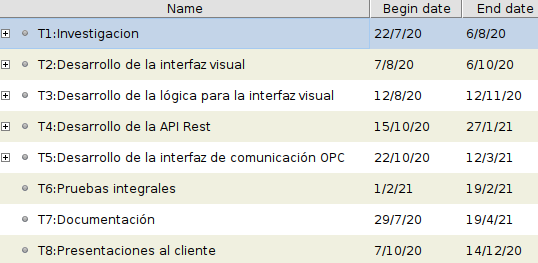
\includegraphics[width=10cm]{gantt_1.png}
 \caption{Tabla con fechas de inicio y fin}
 \label{figure:Tabla}
\end{figure}



\begin{figure}[H]
 \centering
 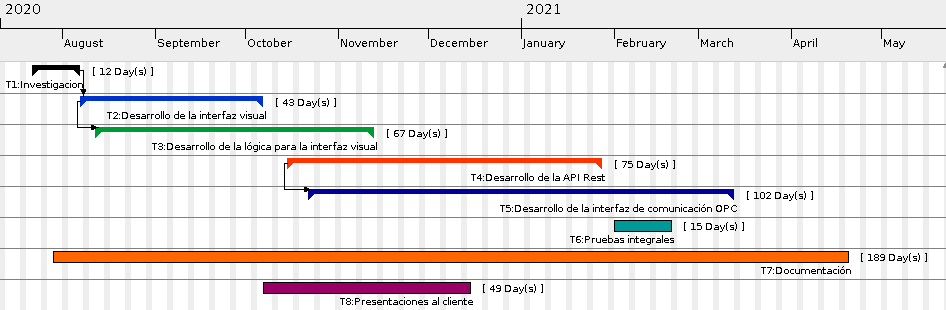
\includegraphics[width=17cm]{gantt_2.png}
 \caption{Diagrama de Gantt}
 \label{figure:Diagrama de Gantt}
\end{figure}

\end{consigna}

\section{9. Matriz de uso de recursos de materiales}
\label{sec:recursos}

\begin{table}[H]
\centering
\setlength\arrayrulewidth{1pt}
\begin{tabular}{|c|c|c|c|}
\hline
\rowcolor[HTML]{CBCEFB} 
\cellcolor[HTML]{CBCEFB}                             & \cellcolor[HTML]{CBCEFB}    & \multicolumn{2}{c|}{\cellcolor[HTML]{CBCEFB} \textbf {Recursos Requeridos}} \\ \cline{3-4} 
\rowcolor[HTML]{CBCEFB} 
\multirow{-2}{*}{\cellcolor[HTML]{CBCEFB} \textbf {Codigo WBS}} & \multirow{-2}{*}{\cellcolor[HTML]{CBCEFB} \textbf {Nombre Tarea}} & \textbf {PC}                          & \textbf {HoloLens2}                          \\ \hline
\cellcolor[HTML]{CBCEFB} T1 & Investigación   &         24        &                      - 				  \\ \hline
\cellcolor[HTML]{CBCEFB} T2 & Desarrollo de la interfaz visual   &         66        &            22            \\ \hline
\cellcolor[HTML]{CBCEFB} T3 & Desarrollo de la lógica para la interfaz visual   &       116          &     20     \\ \hline
\cellcolor[HTML]{CBCEFB} T4 & Desarrollo de la API Rest  &        152         &          -              \\ \hline
\cellcolor[HTML]{CBCEFB} T5 & Desarrollo de la interfaz de comunicación OPC  &        160         &    -  \\ \hline
\cellcolor[HTML]{CBCEFB} T6 & Pruebas integrales &        22         &    10  	\\ \hline
\cellcolor[HTML]{CBCEFB} T7 & Documentación &        32       &        -   	\\ \hline
\cellcolor[HTML]{CBCEFB} T8 & Presentaciones al cliente  &        -         &		16  \\ \hline
\end{tabular}
\end{table}

\section{10. Presupuesto detallado del proyecto}
\label{sec:presupuesto}
El costo total del proyecto es de 3150 USD.

\begin{consigna}{black}
\begin{table}[H]
\setlength\arrayrulewidth{1pt}
\begin{tabular}{|c|c|c|l|}
\hline
\cellcolor[HTML]{CBCEFB}                            & \cellcolor[HTML]{CBCEFB}                           & \multicolumn{2}{c|}{\cellcolor[HTML]{CBCEFB}}                        \\
\multirow{-2}{*}{\cellcolor[HTML]{CBCEFB}\textbf {Categoría}} & \multirow{-2}{*}{\cellcolor[HTML]{CBCEFB} \textbf {Detalle}}  & \multicolumn{2}{c|}{\multirow{-2}{*}{\cellcolor[HTML]{CBCEFB} \textbf {Costo}}} \\ \hline
Trabajo Directo                                     & Valor Hora Responsable Proyecto : 640 hs (2 USD/hs) & \multicolumn{2}{c|}{1208 USD}                                         \\ \hline
Costo Directo                                       & HoloLens2                                          & \multicolumn{2}{c|}{3000 USD}                                        \\ \hline
Costo Indirecto                                     & Viaticos:                              & \multicolumn{2}{c|}{50 USD}                                             \\ \hline
\multicolumn{2}{|c|}{\textbf {Total}}                                                                              & \multicolumn{2}{c|}{\textbf {4258 USD}}                                             \\ \hline
\end{tabular}
\end{table}

\end{consigna}

\section{11. Matriz de asignación de responsabilidades}
\label{sec:responsabilidades}
\begin{consigna}{black}
Se define la asignación de responsabilidades según las siguientes referencias:

\begin{table}[H]
\footnotesize
\setlength\arrayrulewidth{1pt}
\begin{tabular}{|c|c|}
\hline
\cellcolor[HTML]{CBCEFB}                                      & \cellcolor[HTML]{CBCEFB}                               \\
\multirow{-2}{*}{\cellcolor[HTML]{CBCEFB}\textbf{Referencia}} & \multirow{-2}{*}{\cellcolor[HTML]{CBCEFB}\textbf{Rol}} \\ \hline
P                                                             & Responsabilidad Primaria                               \\ \hline
S                                                             & Responsabilidad Secundaria                             \\ \hline
A                                                             & Aprobación                                             \\ \hline
I                                                             & Informado                                              \\ \hline
C                                                             & Consultado                                             \\ \hline
\end{tabular}
\end{table}


\begin{table}[htpb]
\centering
\setlength\arrayrulewidth{1pt}
\resizebox{\textwidth}{!}{%
\begin{tabular}{|c|c|c|c|c|c|}
\hline
\rowcolor[HTML]{CBCEFB} 
\cellcolor[HTML]{CBCEFB} &
  \cellcolor[HTML]{CBCEFB} &
  \multicolumn{4}{c|}{\cellcolor[HTML]{CBCEFB}\textbf {Interesados en el proyecto}} \\ \cline{3-6} 
\rowcolor[HTML]{CBCEFB} 
\cellcolor[HTML]{CBCEFB} &
  \cellcolor[HTML]{CBCEFB} &
  \textbf {Responsable} &
  \textbf {Orientador} &
  \textbf {Equipo} &
  \textbf {Cliente} \\ \cline{3-6} 
\rowcolor[HTML]{CBCEFB} 
\multirow{-3}{*}{\cellcolor[HTML]{CBCEFB}\begin{tabular}[c]{@{}c@{}}\textbf {Código}\\ \textbf{WBS}\end{tabular}} &
  \multirow{-3}{*}{\cellcolor[HTML]{CBCEFB}\textbf {Nombre de la tarea}} &
  \authorname &
  \supname &
  Guillermo Lamana &
  \clientename \\ \hline
T1 & Investigación & P & I & I & C \\ \hline
T2 & Desarrollo de la interfaz visual & P & C & I & A \\ \hline
T3 & Desarrollo de la lógica para la interfaz visual & P & C & I/C & C \\ \hline
T4 & Desarrollo de la API Rest & P & C & - & I \\ \hline
T5 & Desarrollo de la interfaz de comunicación OPC & P & C & I & C \\ \hline
T6 & Pruebas integrales & P & C & I & A \\ \hline
T7 & Documentación & P & C & - & I \\ \hline
T8 & Presentaciones al cliente & P & I & C & A \\ \hline
\end{tabular}%
}
\end{table}

\end{consigna}

\section{12. Gestión de riesgos}
\label{sec:riesgos}

\begin{consigna}{red}
a) Identificación de los riesgos (al menos cinco) y estimación de sus consecuencias:
 
Riesgo 1: detallar el riesgo (riesgo es algo que si ocurre altera los planes previstos)
\begin{itemize}
\item Severidad (S): mientras más severo, más alto es el número (usar números del 1 al 10).\\
Justificar el motivo por el cual se asigna determinado número de severidad (S).
\item Probabilidad de ocurrencia (O): mientras más probable, más alto es el número (usar del 1 al 10).\\
Justificar el motivo por el cual se asigna determinado número de (O). 
\end{itemize}   

Riesgo 2:
\begin{itemize}
\item Severidad (S): 
\item Ocurrencia (O):
\end{itemize}

Riesgo 3:
\begin{itemize}
\item Severidad (S): 
\item Ocurrencia (O):
\end{itemize}


b) Tabla de gestión de riesgos:      (El RPN se calcula como RPN=SxO)

\begin{table}[htpb]
\centering
\begin{tabularx}{\linewidth}{@{}|X|c|c|c|c|c|c|@{}}
\hline
\rowcolor[HTML]{C0C0C0} 
Riesgo & S & O & RPN & S* & O* & RPN* \\ \hline
       &   &   &     &    &    &      \\ \hline
       &   &   &     &    &    &      \\ \hline
       &   &   &     &    &    &      \\ \hline
       &   &   &     &    &    &      \\ \hline
       &   &   &     &    &    &      \\ \hline
\end{tabularx}%
\end{table}

Criterio adoptado: 
Se tomarán medidas de mitigación en los riesgos cuyos números de RPN sean mayores a ....

Nota: los valores marcados con (*) en la tabla corresponden luego de haber aplicado la mitigación.

c) Plan de mitigación de los riesgos que originalmente excedían el RPN máximo establecido:
 
Riesgo 1: Plan de mitigación (si por el RPN fuera necesario elaborar un plan de mitigación).
  Nueva asignación de S y O, con su respectiva justificación:
  - Severidad (S): mientras más severo, más alto es el número (usar números del 1 al 10).
          Justificar el motivo por el cual se asigna determinado número de severidad (S).
  - Probabilidad de ocurrencia (O): mientras más probable, más alto es el número (usar del 1 al 10).
          Justificar el motivo por el cual se asigna determinado número de (O).

Riesgo 2: Plan de mitigación (si por el RPN fuera necesario elaborar un plan de mitigación).
 
Riesgo 3: Plan de mitigación (si por el RPN fuera necesario elaborar un plan de mitigación)

\end{consigna}


\section{13. Gestión de la calidad}
\label{sec:calidad}

\begin{consigna}{red}
Para cada uno de los requerimientos del proyecto indique:
\begin{itemize} 
\item Req \#1: Copiar acá el requerimiento.

Verificación y validación:

\begin{itemize}
\item Verificación para confirmar si se cumplió con lo requerido antes de mostrar el sistema al cliente:\\
Detallar 
\item Validación con el cliente para confirmar que está de acuerdo en que se cumplió con lo requerido:\\
Detallar  
\end{itemize}

\end{itemize}

Tener en cuenta que en este contexto se pueden mencionar simulaciones, cálculos, revisión de hojas de datos, consulta con expertos, etc.

\end{consigna}

\section{14. Comunicación del proyecto}
\label{sec:comunicaciones}

\begin{consigna}{red}
El plan de comunicación del proyecto es el siguiente:
\end{consigna}

% Please add the following required packages to your document preamble:
% \usepackage{graphicx}
% \usepackage[table,xcdraw]{xcolor}
% If you use beamer only pass "xcolor=table" option, i.e. \documentclass[xcolor=table]{beamer}
\begin{table}[htpb]
\centering
\resizebox{\textwidth}{!}{%
\begin{tabular}{|c|c|c|c|c|c|}
\hline
\rowcolor[HTML]{C0C0C0} 
\multicolumn{6}{|c|}{\cellcolor[HTML]{C0C0C0}PLAN DE COMUNICACIÓN DEL PROYECTO}           \\ \hline
\rowcolor[HTML]{C0C0C0} 
¿Qué comunicar? & Audiencia & Propósito & Frecuencia & Método de comunicac. & Responsable \\ \hline
                &           &           &            &                      &             \\ \hline
                &           &           &            &                      &             \\ \hline
                &           &           &            &                      &             \\ \hline
                &           &           &            &                      &             \\ \hline
                &           &           &            &                      &             \\ \hline
\end{tabular}%
}
\end{table}

\section{15. Gestión de Compras}
\label{sec:compras}

\begin{consigna}{red}
En caso de tener que comprar elementos o contratar servicios:
a) Explique con qué criterios elegiría a un proveedor.
b) Redacte el Statement of Work correspondiente.
\end{consigna}

\section{16. Seguimiento y control}
\label{sec:seguimiento}

\begin{consigna}{red}
Para cada tarea del proyecto establecer la frecuencia y los indicadores con los se seguirá su avance y quién será el responsable de hacer dicho seguimiento y a quién debe comunicarse la situación (en concordancia con el Plan de Comunicación del proyecto).

El indicador de avance tiene que ser algo medible, mejor incluso si se puede medir en \% de avance. Por ejemplo,se pueden indicar en esta columna cosas como ``cantidad de conexiones ruteadeas'' o ``cantidad de funciones implementadas'', pero no algo genérico y ambiguo como ``\%'', porque el lector no sabe porcentaje de qué cosa.

\end{consigna}

\begin{table}[!htpb]
\centering
\begin{tabularx}{\linewidth}{@{}|X|X|X|X|X|X|@{}}
\hline
\rowcolor[HTML]{C0C0C0} 
\multicolumn{6}{|c|}{\cellcolor[HTML]{C0C0C0}SEGUIMIENTO DE AVANCE}                                                                       \\ \hline
\rowcolor[HTML]{C0C0C0} 
Tarea del WBS & Indicador de avance & Frecuencia de reporte & Resp. de seguimiento & Persona a ser informada & Método de comunic. \\ \hline
 &  &  &  &  &  \\ \hline
 &  &  &  &  &  \\ \hline
 &  &  &  &  &  \\ \hline
 &  &  &  &  &  \\ \hline
 &  &  &  &  &  \\ \hline
\end{tabularx}%
%}
\end{table}

\section{17. Procesos de cierre}    
\label{sec:cierre}

\begin{consigna}{red}
Establecer las pautas de trabajo para realizar una reunión final de evaluación del proyecto, tal que contemple las siguientes actividades:

\begin{itemize}
\item Pautas de trabajo que se seguirán para analizar si se respetó el Plan de Proyecto original:
 - Indicar quién se ocupará de hacer esto y cuál será el procedimiento a aplicar. 
\item Identificación de las técnicas y procedimientos útiles e inútiles que se utilizaron, y los problemas que surgieron y cómo se solucionaron:
 - Indicar quién se ocupará de hacer esto y cuál será el procedimiento para dejar registro.
\item Indicar quién organizará el acto de agradecimiento a todos los interesados, y en especial al equipo de trabajo y colaboradores:
  - Indicar esto y quién financiará los gastos correspondientes.
\end{itemize}

\end{consigna}


\end{document}
